\chapter{Proverb 4}

\begin{figure}
  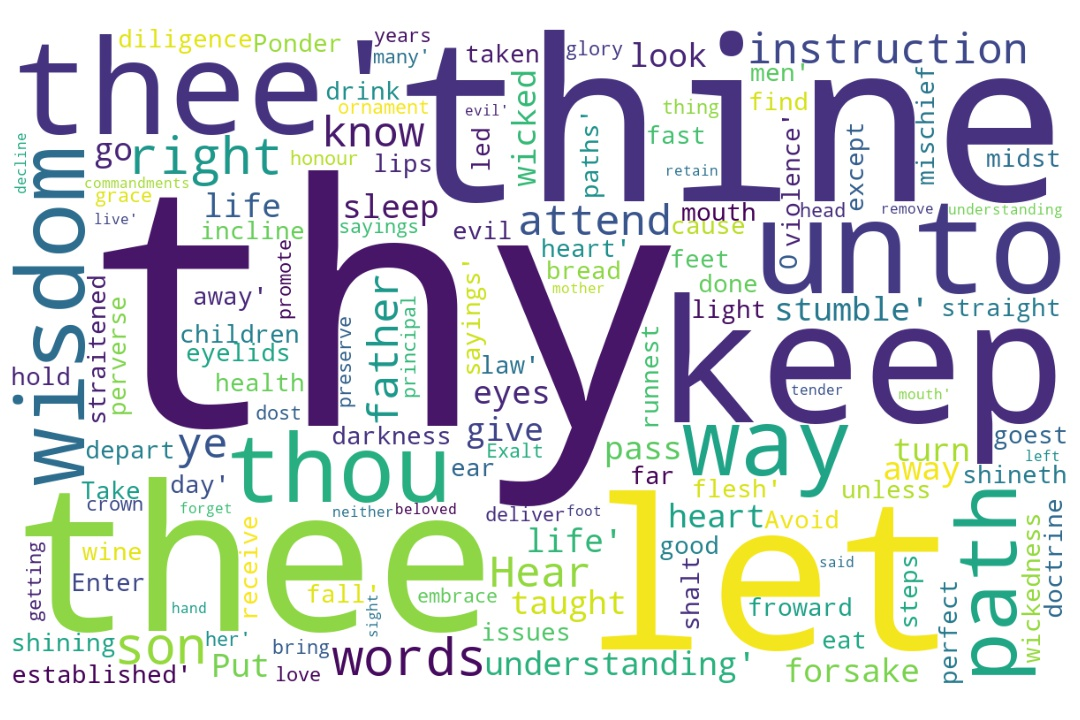
\includegraphics[width=\linewidth]{20OT-Proverbs/Proverb4-WordCloud.jpg}
  \caption{Proverb 4 Word Cloud}
  \label{fig:Proverb 4 Word Cloud}
\end{figure}

% [cmyk]{0.99998,1,0,0}{
%\marginpar{\scriptsize \textcolor[rgb]{0.00,0.545,0.269}{$\rightarrow$7 Princes:  (1) Carshena, (2) Shethar, (3) Admatha, (4) Tarshish, (5) Meres, %(6) Marsena, and (7) Memucan.}}
\marginpar{\scriptsize \centering \fcolorbox{bone}{lime}{\textbf{WHAT WISDOM DOES}}\\ (Proverb 4:1--27) 
\begin{compactenum}[I.][8]
    \item \textbf{Contains Instructions that Liberate} \index[scripture]{Proverbs!Pro 04:13} (Pro 4:13)
    \item \textbf{Corrects Ill-Conceived Lies} \index[scripture]{Proverbs!Pro 04:14-19} (Pro 4:14-19)
    \item \textbf{Counteracts Ill-focused Living} \index[scripture]{Proverbs!Pro 04:14-19} (Pro 4:14-19) 
    \item \textbf{Contains Illuminating Light} \index[scripture]{Proverbs!Pro 04:18}(Pro 4:18) 
    \item \textbf{Condemns the Ignorant Losers} \index[scripture]{Proverbs!Pro 04:19}(Pro 4:19)
    \item \textbf{Covers the Issues of Life} \index[scripture]{Proverbs!Pro 04:22}(Pro 4:22)
    \item \textbf{Challenges Us to Incessant Learning} \index[scripture]{Proverbs!Pro 04:23}(Pro 4:23) 
\end{compactenum} }

\marginpar{\scriptsize \centering \fcolorbox{bone}{yellow}{\textbf{INSTRUCTIONS CONCERNING}}\\
 \fcolorbox{bone}{yellow}{\textbf{WISDOM}} \\ (Proverb 4:1--27) 

\textbf{Introduction}: Scripture has much to say concerning wisdom.
\begin{compactenum}[I.][8]
\item \textbf{Regard It} \index[scripture]{Proverbs!Pro 04:01}(Pro 4:1)
\item \textbf{Retain It} \index[scripture]{Proverbs!Pro 04:04}(Pro 4:4)
\item \textbf{Reach for It} \index[scripture]{Proverbs!Pro 04:05}(Pro 4:5)
\item \textbf{Remember it as a Priority} \index[scripture]{Proverbs!Pro 04:05}(Pro 4:5)
\item \textbf{Reject what is Not Wisdom} \index[scripture]{Proverbs!Pro 04:14--15}(Pro 4:14-15)
\item \textbf{Realise what Wisdom Provides} \index[scripture]{Proverbs!Pro 04:21--22}(Pro 4:21-22)
\item \textbf{Reflect upon the Wisdom of your Ways} \index[scripture]{Proverbs!Pro 04:26}(Pro 4:26)
\end{compactenum} }

\marginpar{\scriptsize \centering \fcolorbox{bone}{black}{\textbf{\textcolor[cmyk]{0,0,0,0}{DESIRING WISDOM}}}\\ (Proverb 4:1--27) 
\begin{compactenum}[I.][8]
    \item \textbf{Realize its Practical Benefits} \index[scripture]{Proverbs!Pro 04:01-27}(Pro 4:1-27)
    \item \textbf{Make it a Priority} \index[scripture]{Proverbs!Pro 04:07} (Pro 4:7)
    \item \textbf{Recognize the Principles of Wisdom} \index[scripture]{Proverbs!Pro 04:01}(Pro 4:1)
    \item \textbf{Expect it to Promote You} \index[scripture]{Proverbs!Pro 04:08, 09}(Pro 4:8, 9) 
    \item \textbf{Expect it to Preserve You} \index[scripture]{Proverbs!Pro 04:22}(Pro 4:22) 
    \item \textbf{Should Be a Preoccupation} \index[scripture]{Proverbs!Pro 04:20-22}(Pro 4:20-22) 
    \item \textbf{Revel in its Presence}  \index[scripture]{Proverbs!Pro 04:08}(Pro 4:8) 
    \item \textbf{Regard it as Precious} \index[scripture]{Proverbs!Pro 04:13}(Pro 4:13) 
\end{compactenum} }

\marginpar{\scriptsize \centering\fcolorbox{black}{blue}{\textbf{\textcolor[cmyk]{0,0,0,0}{KNOWLEDGE, WISDOM}}}\\\fcolorbox{black}{blue}{\textbf{\textcolor[cmyk]{0,0,0,0}{\& UNDERSTANDING}}}\\  \fcolorbox{black}{blue}{\textbf{\textcolor[cmyk]{0,0,0,0}{IN CONTEXT}}}\\ (Proverb 4:1-27) 
\begin{compactenum}[I.][7]
    \item A \textbf{Father's Care} (Pro 4:1)
    \item A \textbf{Faithful Choice} (Pro 4:1-27)
    \item A \textbf{Firm Consideration} (Pro 4:1-27)
    \item A \textbf{First Concern} (Pro 4:7)
    \item A \textbf{Final Crown} (Pro 4:9)
    \item A \textbf{Full Course} (Pro 4:10)
    \item A \textbf{Future Challenge} (Pro 4:5, 6, 7, 8, 13)
\end{compactenum} }

% arginpar{\scriptsize \centering \fcolorbox{bone}{lime}{\textbf{INSTRUCTION CONCERNING WSDOM}}\\ 
% \marginpar{\scriptsize \centering \fcolorbox{bone}{yellow}{\textbf{INSTRUCTIONd CONCERNING WSDOM}}\\ 
% \marginpar{\scriptsize \centering \fcolorbox{bone}{black}{\textbf{\textcolor[cmyk]{0,0,0,0}{DESIRING WISDOM}}}\\ 
% \marginpar{\scriptsize \centering \fcolorbox{black}{blue}{\textbf{\textcolor[cmyk]{0,0,0,0}{GOING TOWARD UNDERSTANDING}}}\\ (Passage) 
% \marginpar{\scriptsize \centering \fcolorbox{black}{ForestGreen}{\textbf{\textcolor[cmyk]{0,0,0,0}{EXAMPLE}}}\\ (Proverbs 4:1-27) 


\footnote{\textcolor[cmyk]{0.99998,1,0,0}{\hyperlink{TOC}{Return to end of Table of Contents.}}}\footnote{\href{https://audiobible.com/bible/bible.html}{\textcolor[cmyk]{0.99998,1,0,0}{Proverbs Audio}}}\textcolor[cmyk]{0.99998,1,0,0}{Hear, ye children, the instruction of a father, and attend to know understanding.}\footnote{\textbf{Proverb 1:8} - My son, hear the instruction of thy father, and forsake not the law of thy mother:}\footnote{\textbf{Proverb 5:1} - My son, attend unto my wisdom, and bow thine ear to my understanding:}\footnote{\textbf{Proverb 8:32-36} - Now therefore hearken unto me, O ye children: for blessed are they that keep my ways. Hear instruction, and be wise, and refuse it not. Blessed is the man that heareth me, watching daily at my gates, waiting at the posts of my doors. For whoso findeth me findeth life, and shall obtain favour of the LORD. But he that sinneth against me wrongeth his own soul: all they that hate me love death.}\footnote{\textbf{Hebrews 2:1} - Therefore we ought to give the more earnest heed to the things which we have heard, lest at any time we should let them slip.}
[2] \textcolor[cmyk]{0.99998,1,0,0}{For I give you good doctrine, forsake ye \fcolorbox{bone}{bone}{not} my law.}
[3] \textcolor[cmyk]{0.99998,1,0,0}{For I was my father's son, tender and only \emph{beloved} in the sight of my mother.}
[4] \textcolor[cmyk]{0.99998,1,0,0}{He taught me also, and said unto me, Let thine heart retain my words: keep my commandments, and live.}
[5] \textcolor[cmyk]{0.99998,1,0,0}{Get wisdom, get understanding: forget \emph{it} \fcolorbox{bone}{bone}{not}; neither decline from the words of my mouth.}
[6] \textcolor[cmyk]{0.99998,1,0,0}{Forsake her \fcolorbox{bone}{bone}{not}, and she shall preserve thee: love her, and she shall keep thee.}
[7] \textcolor[cmyk]{0.99998,1,0,0}{Wisdom \emph{is} the principal thing; \emph{therefore} get wisdom: and with all thy getting get understanding.}
[8] \textcolor[cmyk]{0.99998,1,0,0}{Exalt her, and she shall promote thee: she shall bring thee to honour, when thou dost embrace her.}
[9] \textcolor[cmyk]{0.99998,1,0,0}{She shall give to thine head an ornament of grace: a crown of glory shall she deliver to thee.}
[10] \textcolor[cmyk]{0.99998,1,0,0}{Hear, O my son, and receive my sayings; and the years of thy life shall be many.}
[11] \textcolor[cmyk]{0.99998,1,0,0}{I have taught thee in the way of wisdom; I have led thee in right paths.}
[12] \textcolor[cmyk]{0.99998,1,0,0}{When thou goest, thy steps shall \fcolorbox{bone}{bone}{not} be straitened; and when thou runnest, thou shalt \fcolorbox{bone}{bone}{not} stumble.}
[13] \textcolor[cmyk]{0.99998,1,0,0}{Take fast hold of instruction; let \emph{her} \fcolorbox{bone}{bone}{not} go: keep her; for \fcolorbox{bone}{lime}{she \emph{is} thy life}.}\\
\\
\P \textcolor[cmyk]{0.99998,1,0,0}{\fcolorbox{bone}{lime}{Enter \fcolorbox{bone}{bone}{not}} into the path of the wicked, and go \fcolorbox{bone}{bone}{not} in the way of evil \emph{men}.}
[15] \textcolor[cmyk]{0.99998,1,0,0}{Avoid it, pass \fcolorbox{bone}{bone}{not} by it, \fcolorbox{bone}{lime}{turn from it}, and pass away.}
[16] \textcolor[cmyk]{0.99998,1,0,0}{For they sleep \fcolorbox{bone}{bone}{not}, except they have done mischief; and their sleep is taken away, unless they cause \emph{some} to fall.}
[17] \textcolor[cmyk]{0.99998,1,0,0}{For they eat the bread of wickedness, and drink the wine of violence.}
[18] \textcolor[cmyk]{0.99998,1,0,0}{But the path of the just \emph{is} as the \fcolorbox{bone}{lime}{shining light}, that shineth more and more unto the perfect day.}
[19] \textcolor[cmyk]{0.99998,1,0,0}{The way of the wicked \emph{is} as \fcolorbox{bone}{lime}{darkness}: they know \fcolorbox{bone}{bone}{not} at what they stumble.}\\
\\
\P \textcolor[cmyk]{0.99998,1,0,0}{My son, attend to my words; incline thine ear unto my sayings.}
[21] \textcolor[cmyk]{0.99998,1,0,0}{Let them \fcolorbox{bone}{bone}{not} depart from thine eyes; keep them in the midst of thine heart.}
[22] \textcolor[cmyk]{0.99998,1,0,0}{For \fcolorbox{bone}{lime}{they \emph{are} life} unto those that find them, and health to all their flesh.}\\
\\
\P \textcolor[cmyk]{0.99998,1,0,0}{Keep thy heart with all \fcolorbox{bone}{lime}{diligence}; for out of it \emph{are} the issues of life.}
[24] \textcolor[cmyk]{0.99998,1,0,0}{Put away from thee a froward mouth, and perverse lips put far from thee.}
[25] \textcolor[cmyk]{0.99998,1,0,0}{Let thine eyes look right on, and let thine eyelids look straight before thee.} 
[26] \textcolor[cmyk]{0.99998,1,0,0}{Ponder the path of thy feet, and let all thy ways be established.}
[27] \textcolor[cmyk]{0.99998,1,0,0}{Turn \fcolorbox{bone}{bone}{not} to the right hand nor to the left: remove thy foot from evil.}

\marginpar{\scriptsize \centering \fcolorbox{bone}{orange}{\textbf{GOING TOWARD}}
\fcolorbox{bone}{orange}{\textbf{UNDERSTANDING}}\\ (Proverb 4:1-27) 

\begin{compactenum}[I.][7]
    \item \textbf{Preservation}  \index[scripture]{Proverbs!Pro 04:06} (Pro 4:6)
    \item The \textbf{Principal} Thing \index[scripture]{Proverbs!Pro 04:07} (Pro 4:7)
    \item \textbf{Promotion}  \index[scripture]{Proverbs!Pro 04:08} (Pro 4:8)
    \item \textbf{Paths}  \index[scripture]{Proverbs!Pro 04:14} (Pro 4:14)
    \item A \textbf{Perfect} Day \index[scripture]{Proverbs!Pro 04:18} (Pro 4:18)
    \item  \textbf{Preversity}  \index[scripture]{Proverbs!Pro 04:24} (Pro 4:24)
    \item  \textbf{Ponderings}  \index[scripture]{Proverbs!Pro 04:26} (Pro 4:26)
\end{compactenum} }

